\chapter{Full Network Simulation Experiments}
\label{chp:experiments}

\glsunset{LIF}
\glsunset{AdEx}
\glsunset{ESS}
\glsunset{BiNAM}

This chapter puts the previous theoretical considerations regarding \BiNAM design space exploration and full network evaluation into practice. We finally execute full spiking Willshaw associative memory networks on neuromorphic hardware, assess the predictive power of the single neuron evaluation measures presented in the previous chapter and compare experimental results obtained from different platforms.

In \cref{sec:full_network_software_toolchain}, we discuss the overall methodology for full network simulation. This includes the software framework implemented to this end and an overview of current hardware limitations. \cref{sec:neuron_parameter_sweeps} revisits the neuron parameter sweeps presented in \cref{sec:single_neuron_empirical}. In contrast to the previous experiments, the sweeps are now backed by entire memory networks, either executed on neuromorphic hardware or in software simulation. Finally, \cref{sec:system_parameter_sweeps} presents an analysis of the suitability of \BiNAM system parameter variation as a possible neuromorphic system benchmark.

\section{Methodology and software architecture}
\label{sec:full_network_software_toolchain}

\begin{figure}
	\centering
	\vspace*{1cm}
	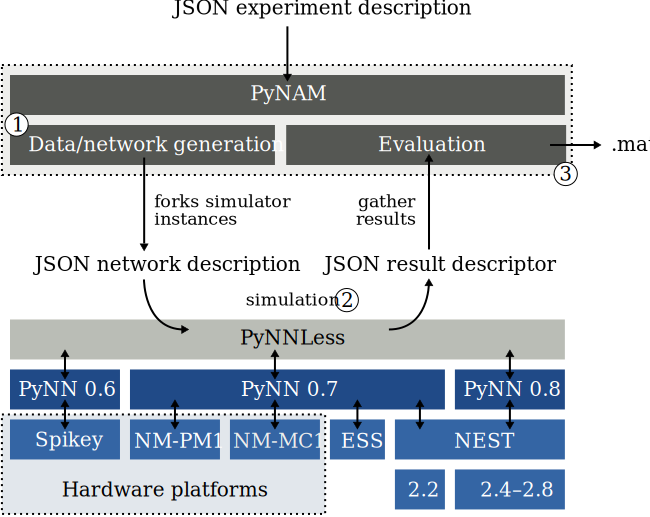
\includegraphics[width=0.9\textwidth]{media/chp5/pynam.pdf}
	\vspace*{0.5cm}
	\caption[Overview of the full network evaluation software stack]{Overview of the software architecture for full network evaluation. The \PyNAM tool generates a series of the network graphs according to a \JSON experiment description file. The serialised, \JSON-like network descriptors are passed to \PyNNLess, a platform agnostic wrapper around the \PyNN framework, which in return passes the recorded results back to \PyNAM, where they are analysed and stored in an \HDF-file (\texttt{.mat}). The encircled numbers refer to the \PyNAM execution stages.}
	\label{fig:pynam}
\end{figure}

In theory, the methodology for the simulation and evaluation of full \BiNAM networks is rather straightforward. Given system and neuron parameters \nParams (\cref{sec:design_space_defn}), a test dataset \data is generated according to \cref{alg:binam_balanced_data}. A \BiNAM memory matrix \memMat is then calculated for this dataset (\cref{eqn:binam_training}). The memory matrix is the basis for the synaptic connections in the network graph (\cref{sec:neural_network_topology}) and the input spikes train descriptors \tIn, \kIn (\cref{alg:input_data_generation}). The network is then executed with the help of the \PyNN abstraction layer (\cref{sec:pynn}) on an arbitrary hardware or software simulator. Finally, the recorded output spike trains \tOut are analysed with respect to the evaluation measures presented in \cref{sec:memory_evaluation_measures}.

For two reasons this approach is not feasible in practice: the first being platform-specific inconsistencies in the \PyNN software layer, and the second an inefficient utilisation of the hardware resources. Two software based solutions were developed to overcome these challenges, \PyNNLess and \PyNAM, which are presented in the following.


\subsection{PyNNLess}
\label{sec:pynnless}

There are -- often minor -- inconsistencies in the implementation of the \PyNN specification for all targeted platforms, for both hardware and software simulators. Furthermore, a total of three consecutive \PyNN versions have to be supported. Each version differs in functionality and semantics
\marginnote{The encountered inconsistencies are most likely due to the early state of the \HBP software stack and are likely to be solved in the next months. The experiments presented in this thesis are the first to run on all \HBP hardware platforms.}
of the provided \API. This renders the use of the exact same code across all platforms difficult. Generally, there are two possible solutions to such a problem. Either the network execution stage in the above pipeline is rewritten for each target platform, or another software abstraction layer is added on top of \PyNN, which levels the discrepancies out.

\marginnote{A short usage example of \PyNNLess is provided in \cref{app:pynnless_example}.}
To avoid redundancies and improve the modularity of the code, the latter approach was chosen for the implementation of experiments on neuromorphic hardware for this thesis. The result of this effort is the \PyNNLess Python library. Its functionality is provided as a data-driven \acrshort{API} \cite{reddy2011api}. The \API receives a network descriptor as a simple data structure, which consists of the neurons and their connectivity as adjacency list, the input spike trains and the signals for recording. After successful network execution, the library returns a data structure containing the recorded output. \PyNNLess supports all \HBP neuromorphic hardware platforms, as well as the \NMPM emulator \ESS and the software simulator \NEST (\cref{fig:pynam}).

\pagebreak


\subsection{PyNAM}
\label{sec:pynam}

\marginnote{To guarantee reproducibility of the test runs, both random data generation and noise sampling must be deterministic -- two executions of \mbox{\PyNAM} should execute the exact same network.}
Construction and evaluation of single \BiNAM instances is a rather modest task and was discussed in staggering detail in \cref{chp:spinam}. In practice however, we need to execute network simulations as part of a system or neuron parameter sweep. Furthermore, due to probabilistic sampling of the test dataset \data and the input spike trains \tIn, as well as potentially noisy analogue hardware systems, single experiments must be repeated multiple times. In the optimal case, the outcome of an experiment should always be a distribution of results. Consequently, a rather large number of individual simulation runs is usually performed for each experiment. Especially when investigating small networks, sequential execution of individual simulations is not an option, as the accumulated pre- and post-processing overhead on the hardware systems would be larger than the execution time itself, while large portions of the hardware resources would lie dormant.

\marginnote{For the execution on single-threaded software simulators \PyNAM generates at least as many experiment groups as the number of {\CPU}s in the system, allowing to execute the experiment groups concurrently on all cores.}
To this end, the \acrlong{PyNAM} (\mbox{\PyNAM}) has been developed. It implements the system parameters and evaluation measures presented in \cref{chp:spinam}, except for input sample pipelining and energy consumption measurements. The tool automatises the process of parameter sweeps and experiment repetition and implements two experiment multiplexing schemes to mitigate the effect of high setup times and to fully utilise available hardware resources. These schemes are \emph{spatial} and \emph{temporal multiplexing}.

\marginnote{For platforms with global neuron parameters (such as Spikey), \PyNAM ensures equality of these parameters within each experiment group.}
Spatial multiplexing is the processes of packing the individual network graphs of independent simulations into a single, concurrently executed graph referred to as \emph{experiment group}. The size of the experiment group is limited by a platform-specific maximum neuron count. While the individual networks in an experiment group are theoretically independent, they may in practice interfere with each other on neuromorphic hardware systems, for example due to congestion of the digital communication network. To mitigate such effects, \PyNAM randomly shuffles the order in which the individual simulations are executed for each repeated run.

\marginnote{The pause between spike trains is chosen as $10 \cdot \timeWindow$, where \timeWindow is sample interval of the last experiment.}
Temporal multiplexing refers to the reuse of the same network graph for a sequence of simulation runs. This is only possible if sweeps over input data encoding parameters are performed (\cref{tbl:design_space}). These solely cause variations in the input datasets, but do not influence the network graph itself. The generated input spike trains corresponding to each individual parameter set are joined into a single compound input spike train by the temporal multiplexing mechanism. Individual parameter sets are separated by a long pause, allowing the neurons to reset. Preceding the analysis, the output spike trains are split into their individual compartments.

\marginnote{An example of the experiment descriptor file is shown in \cref{app:pynam_experiment_json}.}
As indicated in \cref{fig:pynam}, \PyNAM is separated into three phases: construction and serialisation of the experiment groups according to a \JSON experiment description, execution of the experiment groups on the software or hardware simulator and the final demultiplexing and analysis resulting in a single \HDF file \cite{hdf2015website}. The use of \PyNNLess as a middleware allows execution of the experiments on all supported platforms. \PyNAM furthermore automatically adapts the spatial multiplex sizes according the limitations of the current platform.


\subsection{Limitations of the hardware platforms}
\label{sec:neuromorphic_hardware_status}

An overview of the neuromorphic hardware systems and their nominal specifications has been given in \cref{sec:neuromorphic_hardware}. With the exception of Spikey the systems were still in early development at the time of writing. The platforms were neither available in their final size, nor were the software interfaces complete. This results in various limitations regarding the subsequent experiments.

\paragraph{Limitations of NM-MC1}
\marginnote{In \PyNAM the maximum number of neurons is limited to $1\,500$, as the excessive use of population objects in {\PyNAM} disproportionally slows down the place-and-route algorithm.}
Currently the many core system \mbox{\NMMC}, as available to \HBP researchers, consists of three 48-chip boards theoretically allowing the concurrent simulation of more than $100\,000$ individual neurons. However, due to limitations in the place-and-route algorithm regarding population objects and how they are used by \PyNAM, the maximum number of neurons is limited to one per processor core, amounting to about $2100$ \LIF neurons. Apart from this restriction -- which is likely to be resolved in the near future -- the system works as intended.

\paragraph{Limitations of NM-PM1 and ESS}
Unfortunately, the same cannot be said of the physical model \NMPM. While the network basically runs on the platform, known issues with the current revision of the \mbox{\HICANN}-chip cause a rather erratic behaviour of the platform. Due to these issues, no reasonable experiments could be conducted on \NMPM. An older revision of the \NMPM software emulator, the \ESS, is used instead. However, due to detailed hardware emulation, the system is far to slow for two-dimensional parameter sweeps.

\paragraph{Limitations of Spikey}
As already mentioned in \cref{sec:spikey} the single-chip analogue neuromorphic hardware system Spikey \cref{fig:spikey,sec:spikey} has rather severe restrictions regarding the neuron parameter space of its 192~\LIF neurons: the excitatory reversal potential and membrane capacitance are constant at $\Ee = \SI{0}{\milli\volt}$ and $\Cm = \SI{0.2}{\nano\farad}$, and the parameters $\Ei, \ETh, \El, \Ereset$ are shared in blocks of 96 neurons and limited to a maximum of $\SI{-55}{\milli\volt}$. The parameters $\Gl$ and $\TauRef$ can be set individually per neuron. The synapse time constants $\TauE$ and $\TauI$ cannot be provided by the user. They implicitly depend on the synaptic weight \wsyn and the membrane leak conductivity \Gl \cite{pfeil2013six}.

\section{Neuron parameter evaluation}
\label{sec:neuron_parameter_sweeps}

In \cref{sec:single_neuron_empirical}, we performed two neuron parameter sweep experiments aimed at empirical comparison of the single neuron evaluation measures. However, these experiments can not assess the predictive power of single neuron evaluation for the storage capacity \info of entire networks. In this section we aim at bridging this gap by repeating the previous parameter sweeps with full \BiNAM networks instead of single neurons. The full network simulations are performed with \LIF neurons on the software simulator \NEST, and independently on the fully digital \NMMC and analogue Spikey hardware systems. This allows both verification of the single neuron evaluation measures and comparison of the hardware performance to the reference software simulator.

Subsequently, we first elaborate on the experiment methodology, followed by a description of the results for \NMMC and Spikey. Finally, we discus the insights gained from the parameter sweeps.

\subsection{Methodology}
\label{sec:neuron_parameter_sweep_methodology}

\marginnote{This supposedly small network size was chosen in order to limit both the time required for network generation in \PyNAM and the \NEST simulation to sensible ranges.}
Analogously to the parameter sweeps in \cref{sec:single_neuron_empirical}, the initial neuron parameters are selected according to \cref{tbl:initial_parameters}. System parameters which were already relevant for single neuron evaluation follow \emph{Scenario I} in \cref{tbl:scenarios}. Additionally, the network size is selected as $\dimIn = 16$ input signals and $\dimOut = 16$ output neurons, with $\nOnesIn = 3$ one-bits in the input data vectors $\vIn_k$ (as assumed in the single neuron evaluation) and $\nOnesOut = 3$ one-bits in $\vOut_k$.
\marginnote{The optimal input sample count is automatically selected by \PyNAM.}
According to \cref{eqn:binam_entropy,eqn:expected_err} the maximum storage capacity is reached for this data configuration at $\nSamples = 27$ input samples. The particular dataset \data generated by \PyNAM, achieves a maximum storage capacity of $\info = 227\,\mathrm{bit}$ with ten expected false positives over all test samples.

The neuron parameter vectors are sampled from a uniformly spaced $64 \times 64$ grid. For each parameter vector, the false positive and negative counts \nFP, \nFN, the information measure \info, and the average latency \latency per sample are calculated. Information measure and false negative/positive counts are normalised, to allow direct comparison of the information \info with the single neuron evaluation measures and to improve the comparability of full network evaluations based on distinct system parameters.
\marginnote{The false positive normalisation is only piecewise linear: there are $10$ expected false positives, but $351$ possible false positives. Correspondingly $[0, 10]$ is mapped to $[-1, 0]$ and $[10, 351]$ to $[0, 1]$.}
The false positive count \nFP is normalised to the range $[-1, 1]$, where $\nFP = -1$ corresponds to \enquote{none of the expected false positives are generated}, $\nFP = 0$ to \enquote{the expected number of false positives was generated} and $\nFP = 1$ to \enquote{all bits is in the output were set to one}.  False negative count and information are expressed relative to the maximum possible false negative count and the maximum information respectively.

\subsection{Neuron parameter sweep on NM-MC1}
\label{sec:neuron_parameter_sweep_nmmc}

\begin{figure}[t]
	\centering
	\subbottom[Relative information \info (NEST)]{%
		\includegraphics[trim=2mm 3mm 2mm 2.2mm,clip]{media/chp5/nmmc/plot_0_info_n_2d_nest_small.pdf}%
		\label{fig:exp_info_nestI}
	}%
	\subbottom[Relative information \info (NM-MC1)]{%
		\includegraphics[trim=7mm 3mm 2mm 2.2mm,clip]{media/chp5/nmmc/plot_0_info_n_2d_spiNNaker_small.pdf}%
		\label{fig:exp_info_nmmcI}
	}
	\subbottom[Parameter optimality \Pgen (\STII)]{%
		\includegraphics[trim=2mm 3mm 2mm 2.2mm,clip]{media/chp5/nmmc/i3_ex_nm_Train_N100_XgL_YtauE_pBin_Train_IfCondExp_small.pdf}%
		\hspace{3.9mm}%
		\label{fig:exp_stI}
	}%
	\subbottom[Parameter optimality \Pgen (SGMO)]{%
		\includegraphics[trim=7mm 3mm 2mm 2.2mm,clip]{media/chp5/nmmc/i5_ex_nm_SgMo_XgL_YtauE_pSoft_SgMo_IfCondExp_small.pdf}%
		\hspace{3.9mm}%
		\label{fig:exp_sgmoI}
	}
	\hspace*{7mm}\includegraphics{media/chp5/colorbar_info.pdf}
	{\footnotesize Relative information \info/Parameter optimality \Pgen}
	\caption[First NM-MC1 and NEST neuron parameter sweep]{Comparison of the \Gl/\TauE sweep on the \NEST and \NMMC platforms with the single neuron evaluation results. Refer to \cref{sec:neuron_parameter_sweep_methodology,sec:neuron_parameter_sweep_nmmc} for more information.}
	\label{fig:exp_sweepI}
\end{figure}

\begin{figure}[t]
	\centering
	\subbottom[Relative information \info (\NEST)]{%
		\includegraphics[trim=2mm 3mm 2mm 2.2mm,clip]{media/chp5/nmmc/plot_1_info_n_2d_nest_small.pdf}%
		\label{fig:exp_info_nestII}
	}%
	\subbottom[Relative information \info (\NMMC)]{%
		\includegraphics[trim=7mm 3mm 2mm 2.2mm,clip]{media/chp5/nmmc/plot_1_info_n_2d_spiNNaker_small.pdf}%
		\label{fig:exp_info_nmmcII}
	}
	\subbottom[Parameter optimality \Pgen (\STII)]{%
		\includegraphics[trim=2mm 3mm 2mm 2.2mm,clip]{media/chp5/nmmc/i13_ex_nm_Train_N100_XeTh_Yw_pBin_Train_IfCondExp_small.pdf}%
		\hspace{4.1mm}%
		\label{fig:exp_stII}
	}%
	\subbottom[Parameter optimality \Pgen (\SGMO)]{%
		\includegraphics[trim=7mm 3mm 2mm 2.2mm,clip]{media/chp5/nmmc/i15_ex_nm_SgMo_XeTh_Yw_pSoft_SgMo_IfCondExp_small.pdf}%
		\hspace{4.1mm}%
		\label{fig:exp_sgmoII}
	}
	\hspace*{7mm}\includegraphics{media/chp5/colorbar_info.pdf}
	{\footnotesize Relative information \info/Parameter optimality \Pgen}
	\caption[Second NM-MC1 and NEST neuron parameter sweep]{Comparison of the \ETh/\wsyn sweep on the \NEST and \NMMC platforms with the single neuron evaluation results. Refer to \cref{sec:neuron_parameter_sweep_methodology,sec:neuron_parameter_sweep_nmmc} for more information.}
	\label{fig:exp_sweepII}
\end{figure}

\begin{figure}[p]
	\centering
	\small
	\subbottom[False positives \nFP (\NEST)]{%
		\includegraphics[trim=2mm 3mm 2mm 2.2mm,clip]{media/chp5/nmmc/plot_1_fp_n_2d_nest_small.pdf}%
		\label{fig:exp_fp_nest}
	}%
	\subbottom[False positives \nFP (\NMMC)]{%
		\includegraphics[trim=7mm 3mm 2mm 2.2mm,clip]{media/chp5/nmmc/plot_1_fp_n_2d_spiNNaker_small.pdf}%
		\label{fig:exp_fp_nmmc}
	}
	\subbottom[False negatives \nFN (\NEST)]{%
		\includegraphics[trim=2mm 3mm 2mm 2.2mm,clip]{media/chp5/nmmc/plot_1_fn_n_2d_nest_small.pdf}%
		\label{fig:exp_fn_nest}
	}%
	\subbottom[False negatives \nFN (\NMMC)]{%
		\includegraphics[trim=7mm 3mm 2mm 2.2mm,clip]{media/chp5/nmmc/plot_1_fn_n_2d_spiNNaker_small.pdf}%
		\label{fig:exp_fn_nmmc}
	}
	\hspace*{5.5mm}\includegraphics{media/chp5/colorbar_fp_fn.pdf}
	{\footnotesize Normalised false positive/negative count}
	\subbottom[Latency \latency (\NEST)]{%
		\includegraphics[trim=2mm 3mm 2mm 2.2mm,clip]{media/chp5/nmmc/plot_1_lat_avg_2d_nest_small.pdf}%
		\label{fig:exp_lat_nest}
	}%
	\subbottom[Latency \latency (\NMMC)]{%
		\includegraphics[trim=7mm 3mm 2mm 2.2mm,clip]{media/chp5/nmmc/plot_1_lat_avg_2d_spiNNaker_small.pdf}%
		\label{fig:exp_lat_nmmc}
	}
	\hspace*{7.5mm}\includegraphics{media/chp5/colorbar_lat1.pdf}
	{\footnotesize Average latency \latency [\si{\milli\second}]}
	\caption[NM-MC1 and NEST errors and latencies]{Comparison of the latencies, false positive and false negative counts for the \ETh/\wsyn sweep on \NEST and \NMMC. Refer to \cref{sec:neuron_parameter_sweep_methodology,sec:neuron_parameter_sweep_nmmc} for more information.}
	\label{fig:exp_sweepIIb}
\end{figure}

\marginnote{The results for \SGSO are not compared. Interested readers are referred to the corresponding data in \cref{app:evaluation_measure_comparison}.}
The first parameter sweep executed on \NMMC varies \Gl from \SIrange{0.01}{0.2}{\micro\siemens} and \TauE from \SIrange{0}{20}{\milli\second}. Most strikingly, the results for the \NEST software simulation and the \NMMC neuromorphic hardware (\cref{fig:exp_info_nestI,fig:exp_info_nmmcI}) are almost identical. The region with high optimality in the \STII single neuron evaluation measure (\cref{fig:exp_stI}) overlaps well with the high-information regions in the full network-evaluation. However, \STII slightly overestimates the parameter quality. The same is true for the \SGMO measure (\cref{fig:exp_sgmoI}) which is shifted too far towards larger $\Gl$ compared to \STII.

Minor discrepancies between \NEST and \NMMC can be found in the second parameter sweep, which varies \wsyn from \SIrange{0.01}{0.2}{\micro\siemens} and \TauE from \SIrange{0}{20}{\milli\second}. As shown in \cref{fig:exp_info_nestII}, the region of maximal information is minimally larger on \NEST than on \mbox{\NMMC} (\cref{fig:exp_info_nmmcII}). \STII is again too optimistic in comparison to the ground truth provided by \NEST (\cref{fig:exp_stII}). \SGMO is shifted towards smaller \wsyn, yet exhibits a gradient leading to a global maximum in the region in which \NEST shows the highest information.

Comparison of the false positive and false negative counts for the second sweep in \cref{fig:exp_fp_nest,fig:exp_fp_nmmc,fig:exp_fn_nest,fig:exp_fn_nmmc} shows no striking difference between \NEST and \NMMC apart from a marginally smaller false positive count for \NEST in the region of maximal information. The largest discrepancies between \NEST and \NMMC can be found in  \cref{fig:exp_lat_nest,fig:exp_lat_nmmc}, which contain the latency plots. Whereas \NEST exhibits a smooth wavy grain pattern, the same pattern is interspersed with noise on \NMMC.

\subsection{Neuron parameter sweep on Spikey}
\label{sec:neuron_parameter_sweep_spikey}

\begin{figure}[p]
	\centering
	\small
	\subbottom[Relative information \info (NEST)]{%
		\includegraphics[trim=2mm 3mm 2mm 2.2mm,clip]{media/chp5/spikey/plot_0_info_n_2d_nest_small.pdf}%
		\label{fig:exp2_info_nest}
	}%
	\subbottom[Relative information \info (Spikey)]{%
		\includegraphics[trim=7mm 3mm 2mm 2.2mm,clip]{media/chp5/spikey/plot_0_info_n_2d_spikey_small.pdf}%
		\label{fig:exp2_info_spikey}
	}
	\subbottom[Parameter optimality \Pgen (\STII)]{%
		\includegraphics[trim=2mm 3mm 2mm 2.2mm,clip]{media/chp5/spikey/i3_ex_spikey_Train_N100_XeTh_Yw_pBin_Train_IfCondExp_small.pdf}%
		\label{fig:exp2_st}
	}%
	\subbottom[Parameter optimality \Pgen (SGMO)]{%
		\includegraphics[trim=7mm 3mm 2mm 2.2mm,clip]{media/chp5/spikey/i5_ex_spikey_SgMo_XeTh_Yw_pSoft_SgMo_IfCondExp_small.pdf}%
		\label{fig:exp2_sgmo}
	}
	\hspace*{7mm}\includegraphics{media/chp5/colorbar_info.pdf}
	{\footnotesize Relative information \info/Parameter optimality \Pgen}
	\subbottom[False positives \nFP (\NEST)]{%
		\includegraphics[trim=2mm 3mm 2mm 2.2mm,clip]{media/chp5/spikey/plot_0_fp_n_2d_nest_small.pdf}%
		\label{fig:exp2_fp_nest}
	}%
	\subbottom[False positives \nFP (Spikey)]{%
		\includegraphics[trim=7mm 3mm 2mm 2.2mm,clip]{media/chp5/spikey/plot_0_fp_n_2d_spikey_small.pdf}%
		\label{fig:exp2_fp_spikey}
	}
	\hspace*{5.5mm}\includegraphics{media/chp5/colorbar_fp_fn.pdf}
	{\footnotesize Normalised false positive count \nFP}
	\caption[Spikey parameter sweep overview]{Comparison of the \ETh/\wsyn sweep on the \NEST and Spikey platforms with the single neuron evaluation results and false positive counts. Refer to \cref{sec:neuron_parameter_sweep_methodology,sec:neuron_parameter_sweep_spikey} for more information.}
	\label{fig:exp2_sweepI}
\end{figure}

\begin{figure}
	\centering
	\small
	\subbottom[Latency \latency (\NEST)]{%
		\includegraphics[trim=2mm 3mm 2mm 2.2mm,clip]{media/chp5/spikey/plot_0_lat_avg_2d_nest_small.pdf}%
		\label{fig:exp2_lat_nest}
	}%
	\subbottom[Latency \latency (Spikey)]{%
		\includegraphics[trim=7mm 3mm 2mm 2.2mm,clip]{media/chp5/spikey/plot_0_lat_avg_2d_spikey_small.pdf}%
		\label{fig:exp2_lat_spikey}
	}
	\hspace*{7.5mm}\includegraphics{media/chp5/colorbar_lat2.pdf}
	{\footnotesize Average latency \latency [\si{\milli\second}]}
	\caption[Spikey parameter sweep latencies]{Latencies measured during the Spikey parameter sweep in comparison with the \NEST simulation. Contour lines were not drawn in (b) for a better overview. Refer to \cref{sec:neuron_parameter_sweep_methodology,sec:neuron_parameter_sweep_spikey} for more information.}
	\label{fig:exp2_sweepIb}
\end{figure}

The excitatory channel time constant \TauE is not user-definable on Spikey. Correspondingly, the \Gl/\TauE sweep cannot be performed. The threshold potential \ETh is furthermore limited to a maximum of \SI{-55}{\milli\volt}, which lies outside the range of the previous sweep. A maximally large range (with respect to $\El$ at \SI{-70}{\milli\volt}) is chosen instead and \ETh is varied from \SIrange{-69}{-55}{\milli\volt}. The synaptic channel amplitude is reduced along with \ETh by lowering the \wsyn-range to \SIrange{0.0}{0.016}{\micro\siemens}. Note that the membrane capacitance of Spikey is $\Cm = \SI{0.2}{\nano\farad}$ instead of the previously used $\SI{1.0}{\nano\farad}$.

The results of the parameter sweep on Spikey are shown in \cref{fig:exp2_sweepI,fig:exp2_sweepIb}. In contrast to the previous experiments, the storage capacity measure differs significantly between the software simulator \NEST and the neuromorphic hardware (\cref{fig:exp2_info_nest,fig:exp2_info_spikey}). In the \NEST simulation the region of highest information is spread along a straight line, a behaviour once again reproduced by both \STII and \SGMO, though the results for \SGMO are skewed towards smaller \wsyn (\cref{fig:exp2_st,fig:exp2_sgmo}). Both \NEST and the single neuron evaluation measures coherently indicate that the theoretical maximum information/optimality cannot be reached for the given parameters. The information graph for Spikey is distorted, extremely noisy and has a smaller maximum information than the \NEST simulation.

The comparison of the false positive measure between \NEST and Spikey in \cref{fig:exp2_fp_nest,fig:exp2_fp_spikey} bears another interesting detail. Whereas a graduated transition from regions with negative \nFP (regions with too few output spikes) to regions with positive \nFP (regions with too many output spikes) is present in the false positive count for \NEST, such a transition is almost completely missing on Spikey. The system either produces no Spikes at all or too many spikes. Furthermore, the latency measure in \cref{fig:exp2_sweepIb} shows severe noise and larger latency for Spikey compared to \NEST.


\subsection{Discussion}
\label{sec:neuron_parameter_sweep_discussion}

Above all, the experiments highlight two facts. Firstly, the spiking neural network implementation of the Willshaw associative memory described in \cref{chp:spinam} is operational on neuromorphic hardware, albeit the results for Spikey are suboptimal. In contrast, the neuron parameter sweep on \NMMC found an entire region in the parameter space which achieves the theoretical maximum storage capacity (\cref{fig:exp_info_nmmcI}). Secondly, the single neuron evaluations cohere extremely well with the full network storage capacity measure \info as calculated by the reference network simulator \NEST. This supports the conjecture put forth in \cref{chp:neuron_evaluation}: analysis of a single neuron in the network is sufficient to predict the performance of the full network. Nevertheless, as mentioned in the last chapter, further research is required to correct the slightly deviating behaviour of the otherwise promising \SGMO measure.

The experiments show that \NMMC implements the reference \LIF neuron model extremely well. With the results of the differential equation integrator benchmark in \cref{sec:integrator_benchmark} in mind, the minor deviations from the reference are well explainable with the constant $\stepSize = \SI{1}{\milli\second}$ step size in the \NMMC numerical neuron integrator. The fact that all spikes in \NMMC are discretised to a one-millisecond grid furthermore explains the noise in the memory latency.

The results for the analogue Spikey system are less fortunate. Even though it is visible that Spikey approximately follows the behaviour of the reference, the result is superimposed with severe noise. Possibly, the use of neuron populations might improve the situation, as these theoretically lessen the impact of single noisy neurons (\cref{sec:neuron_populations}). Nevertheless, the main advantage of analogue neuromorphic hardware must not be kept out of sight. Spikey is extremely fast: execution of the above parameter sweep took about ten minutes on Spikey, forty minutes on \NMMC and five hours on \NEST, including all network generation and analysis overhead. More complex biologically inspired networks might not be as susceptible to noise as the \BiNAM. However, it is exactly this susceptibility to noise or other deviations from the norm which suggest that the \BiNAM is a helpful benchmarking network for neuromorphic platforms.


\section{System parameter sweeps}
\label{sec:system_parameter_sweeps}

While the above two-dimensional neuron parameter sweeps are clearly suitable as a benchmark, their computation is rather time consuming and the resulting three-dimensional graphs are hard to analyse. Of course, an intriguingly simple way of comparing two platforms is to just calculate the storage capacity for a constant neuron and system parameter set. However, these parameters must possess a sufficiently large discriminatory power: they should neither pose a barely solvable nor a too trivial problem. A solution to this dilemma is to perform a system parameter sweep which constructs a series of gradually more difficult tests.

This idea is the basis of the so far not tested robustness measure (\cref{sec:eval_robustness}), which sweeps over an arbitrary noise parameter $\sigma$, and the critical time window analysis (\cref{sec:eval_latency}), which varies the  time window \timeWindow. In this section we analyse these measures with respect to their suitability as hardware benchmark. To this end, exemplary one-dimensional system parameter sweeps are performed on the \NEST software simulator, the \NMMC digital neuromorphic hardware system, \ESS as a replacement for \NMPM and Spikey as an analogue neuromorphic hardware system. As before, we begin with a short description of the methodology, followed by the results and a discussion.

\subsection{Methodology}
\label{sec:initial_parameters}

The one dimensional system parameter sweeps performed in this section measure the storage capacity \info over a system parameter. The initial system and neuron parameters are those already employed in the previous experiments. Their description can be found in \cref{sec:neuron_parameter_sweep_methodology}.

To ensure a maximal value range for \info, the neuron parameters \nParams must be optimised prior to the experiment with respect to the initial system parameters. To bear any meaning as a benchmark, the optimisation process targets the reference platform (\NEST), and the neuron parameters \nParams are shared across all platforms. To this end, the Spikey neuron parameter space, a strict subset of the parameter spaces of the other platforms, must be used in the neuron parameter selection. The \LIF neuron membrane capacitance and threshold potential are correspondingly set to $\Cm = \SI{0.2}{\nano\farad}$ and $\ETh = \SI{-55}{\milli\volt}$. According to the neuron parameter sweep in \cref{fig:exp2_info_nest}, a maximum in the storage capacity is reached for $\wsyn = \SI{16}{\nano\siemens}$. A preliminary test run on \NEST shows that these parameters reach the theoretical maximum storage capacity if the spike time jitter is reduced from $\jitter = \SI{5}{\milli\second}$ to $\SI{2}{\milli\second}$ in the initial system parameters.

In the following, the system parameters $\jitter$, $\jitterWSyn$ and $\timeWindow$ are linearly sampled from a given value range in fifty steps. For each sample, the memory storage capacity \info is measured in eight independent runs, over which mean and standard deviation of \info are calculated.

\subsection{Experimental results}

\begin{figure}[t]
	\centering
	\subbottom{%
		\includegraphics[trim=2mm 2mm 2mm 2mm,clip]{media/chp5/system_sweep/plot_1_info.pdf}%
	}
	\subbottom{%
		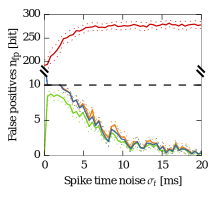
\includegraphics[trim=2mm 2mm 2mm 2mm,clip]{media/chp5/system_sweep/plot_1_fp.pdf}%
	}%
	\subbottom{%
		\hspace{2mm}
		\includegraphics[trim=1.5mm 2mm 2mm 2mm,clip]{media/chp5/system_sweep/plot_1_fn.pdf}%
	}
	\caption[Results of the spike time noise parameter sweep]{Results of the spike time noise parameter sweep. Shown are the information and the corresponding false positive/false negative counts. Solid lines correspond to the mean over eight runs, dotted lines to the $\pm0.5 \cdot \sigma$ standard deviation. The dashed lines show the maximum information and the expected false positive count respectively.}
	\label{fig:exp3_jitter}
\end{figure}

\begin{figure}[t]
	\centering
	\subbottom{%
		\includegraphics[trim=2mm 2mm 2mm 2mm,clip]{media/chp5/system_sweep/plot_2_info.pdf}%
	}
	\subbottom{%
		\includegraphics[trim=2mm 2mm 2mm 7mm,clip]{media/chp5/system_sweep/plot_0_info.pdf}%
	}
	\caption[Results of the synaptic weight noise and time window sweeps]{Results of the spike time noise and time window sweeps showing the information \info over the system parameters. Solid lines correspond to the mean over eight runs, dotted lines to the $\pm0.5 \cdot \sigma$ standard deviation. The dashed line shows the maximum information.}
\end{figure}

In the first experiment, the standard deviation of the Gaussian spike time noise \jitter is varied from \SIrange{0}{20}{\milli\second}. The results are shown in \cref{fig:exp3_jitter}. As expected, the information measure decreases with increasing \jitter. \NEST and \NMMC exhibit a very similar behaviour: both start with the theoretical maximum information and slowly decrease towards zero information. Interestingly, \ESS begins with zero information at $\jitter = \SI{0}{\milli\second}$ and rapidly reaches a relatively large yet not maximal \info at $\jitter = \SI{2}{\milli\second}$. It then converges towards the result for \NEST and \NMMC. Spikey starts with a small \info and converges to a value which is slightly larger than the final result of the other measures.

Comparison of the false positive and false negative counts shows that \NEST, \NMMC and \ESS exhibit a similar overall behaviour with a decreasing false positive count and an increasing false negative count. The zero information at $\jitter = \SI{0}{\milli\second}$ for \ESS is caused by a maximally large initial false negative count $\nFN = 81$. Spikey exhibits a different behaviour, with an increasing false positive count and a constant zero false negative count.

\cref{fig:exp3_jitter} shows the information measure as a result of the sweep over the synapse weight noise \jitterWSyn (from \SIrange{0.0}{10.0}{\nano\siemens}) and the time window \timeWindow (from \SIrange{2}{20}{\milli\second}). Unsurprisingly, the information measure decreases with increasing synapse weight noise for \NEST and \NMMC. Surprisingly, \ESS exhibits very small values over the entire sweep with a large standard deviation. For Spikey, the information starts at a small value and unexpectedly increases slightly with larger noise values. 

The time window analysis exhibits the behaviour that was anticipated in \cref{sec:eval_latency}, with a coherent decrease in the information for smaller time windows $\timeWindow$. Systematic differences in the performances of the platforms are clearly visible.

\subsection{Discussion}
\label{sec:system_parameter_sweep_discussion}

Just like the two-dimensional neuron parameter sweeps, the one dimensional system parameter sweeps are a valuable benchmark. They show a clear separation between models with reference behaviour on the one hand (\NEST and \NMMC), and Spikey and \ESS on the other hand. In two of the sweeps the performance exhibited by \ESS is close to the performance of \NEST and \NMMC, and significantly better than the erratic performance displayed by Spikey, which is -- as in the previous experiment -- characterised by a tremendously large false positive count.

Furthermore, the sweeps uncover suboptimal and interesting behaviour of the platforms. Strikingly and for unknown reasons, ever so slight variations in the synaptic weight cause a breakdown of \ESS performance. The same is true for zero spike time noise. However, a plausible explanation for this behaviour exists: the platform seems to fuse input spikes arriving at the exact same time. Since all spikes arrive at the same time for $\jitter = \SI{0}{\milli\second}$, the neuron produces no output spikes and thus exhibits the large false negative count.

However, the results also show that care has to be taken regarding the range of the sweep. In case platforms show an erratic behaviour they may achieve a larger \info as platforms with a systematic behaviour, as it is the case for the for large \jitter, for which Spikey exhibits a slightly larger \info than the other platforms.


\section{Conclusion}

In this chapter we have presented the software pipeline for full network evaluation. This pipeline has been employed to conduct two sets of experiments on both neuromorphic hardware and in software simulation. The first set of experiments confirmed the predictive power of single neuron evaluation, found a high accordance between the results from \NMMC and \NEST, and a certain dissonance between the results for \NEST and Spikey. The second experiment was similarly capable of discriminating between the individual simulation platforms. As such, the \BiNAM is well suited as a benchmarking network.

Most important, yet almost unmentioned, is the fact, that the primary goal of this thesis -- the implementation of an operational Willshaw associative memory as spiking neural network on neuromorphic hardware -- has been reached. Correspondingly, we can now proceed to the final chapter.
